%==================================================================FRONT PAGE AND TOC
% For article only
\mode<presentation:0>{\thispagestyle{empty}\maketitle}

% For presentation only
\mode<presentation| article:0| handout:0>{
    \begin{frame}<article:0>[label=portada]
    \titlepage
    \end{frame}%Fin del frame
}

% For handout only
\mode<handout>{
  \begin{frame}[label=portada]
    \maketitle
  \end{frame}
}

% %% TABLE OF CONTENTS
% \begin{frame}[label=toc]
%     \mode<article:0>{\frametitle{Contents}}
%     \mode<presentation>{\small}
%     \tableofcontents[hidesubsections]
% \end{frame}

\begin{frame}[label=portada]
 \titlepage
\end{frame}
\begin{frame}[label=toc]
  \frametitle{Resumen}
\tableofcontents[hidesubsections]
\end{frame}
% \rowcolors{1}{ZurichBlue!20}{ZurichBlue!5}
%%==================================================================S INTRODUCTION
\section{Herramientas}
%%==================================================================F 
\begin{frame}
    \frametitle{Herramientas}
    \begin{enumerate}
        \item GRASS LiDAR tools 
	\begin{itemize}
            \item \texttt{v.outlier}
            \item \texttt{v.lidar.edgedetetion}
            \item \texttt{v.lidar.growing}
            \item \texttt{v.lidar.correction}
            \item \texttt{v.surf.bspline}
	\end{itemize}
        \item LibLAS
	\begin{itemize}
            \item \texttt{las2las}, \texttt{las2txt}, \texttt{txt2las}, \texttt{lasdiff}, \texttt{lasinfo} 
	\end{itemize}
        \item LAStools
	\begin{itemize}
            \item \texttt{las2las}, \texttt{las2txt}, \texttt{txt2las},
                \texttt{shp2las}, \texttt{lasground}, \texttt{las2dem}, \texttt{txt2tin}
	\end{itemize}
        \item PCL (Point Cloud Library)
        \item PDAL (Point Data Abstraction Library)
    \end{enumerate}
\end{frame}
%%==================================================================S
\section{Análisis LiDAR en GRASS}
%%==================================================================Sb
\begin{frame}
    \frametitle{Geographic Resources Analysis Support System\hfill
        
\includegraphics[width=0.7cm]{images/grasslogo_transp_big.png}} 
     \begin{itemize}
        \item Conocido como \alert<1>{GRASS}: GIS para manipulación y
            análisis de datos geoespaciales.
        \item Como es un programa de \alert{códico abierto} con un montón de
            librerias, es muy adecuado para la implementación de nuestras
            propias herramientas.
        \item Escrito en C/C++, lo que permite implementar programas
            computacionalmente pesados $\Rightarrow$ \alert{ideal} para trabajar
            con LiDAR.
        \item GRASS $\geq$ 6 incluye indexación topológica $\Rightarrow$
            \alert{fatal} para trabajar con LiDAR.  \item Hay versiones para
            GNU/Linux, MS-Windows, Mac-OSX, SUN, etc.
            \alert{\textexclamdown\textexclamdown Todos lo pueden utilizar!!}
        \item Más información en:
            \beamergotobutton{\url{http://grass.osgeo.ogr}}
    \end{itemize}
\end{frame}
%%==================================================================Sb
\subsection{Importando nube de puntos}
%%==================================================================F 
\begin{frame}
 \frametitle{Importar como raster: \LARGE\path{r.in.xyz}}
\end{frame}
%%==================================================================F 
\begin{frame}
 \frametitle{Importar como vectorial: \LARGE\path{v.in.ascii}}
\end{frame}
%%==================================================================Sb
\subsection{GRASS LiDAR tools}
\begin{frame}
  \frametitle{GRASS LiDAR tools}
  Eliminación de objetos en nubes de puntos y creación de MDT's
  \begin{minipage}{0.45\textwidth}
  \begin{itemize}
    \item<2-> \path{v.outlier}
    \item<3-> \path{v.lidar.edgedetection}
    \item<4-> \path{v.lidar.growing}
    \item<5-> \path{v.lidar.correction}
    \item<6-> \path{v.surf.bspline}
  \end{itemize}
  \end{minipage}
  \begin{minipage}{0.45\textwidth}
    \begin{picture}(275,110)
    \uncover<3->{\put(0,0){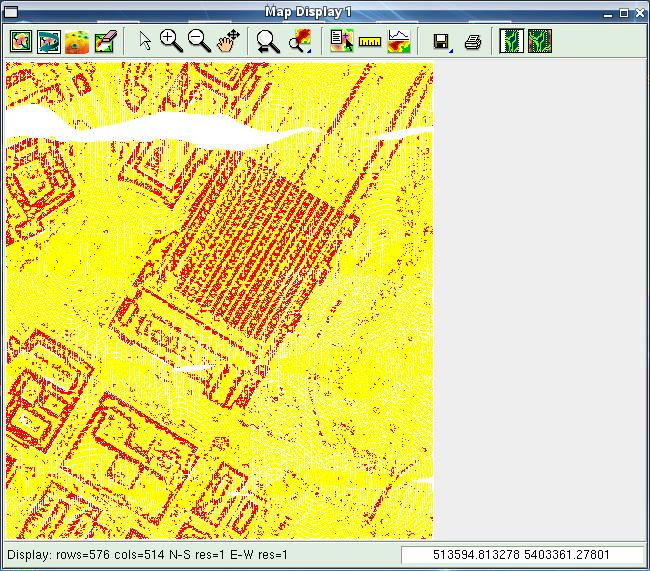
\includegraphics[width=0.75\textwidth]{images/edge}}}
    \uncover<4->{\put(10,-10){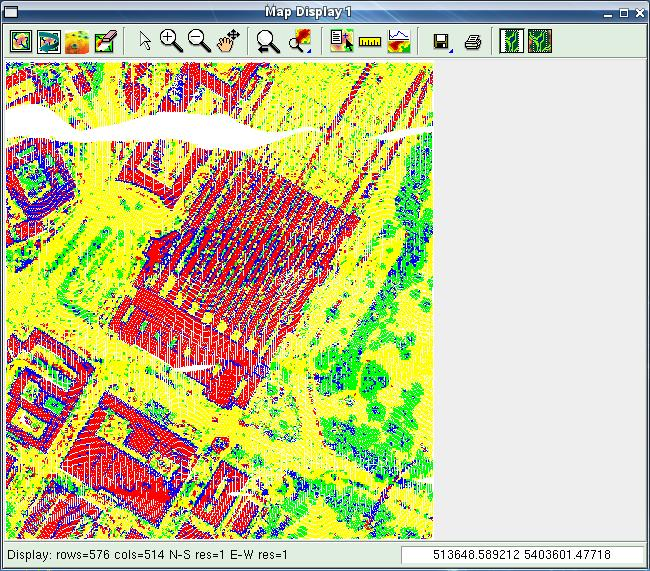
\includegraphics[width=0.75\textwidth]{images/grow}}}
    \uncover<5->{\put(20,-20){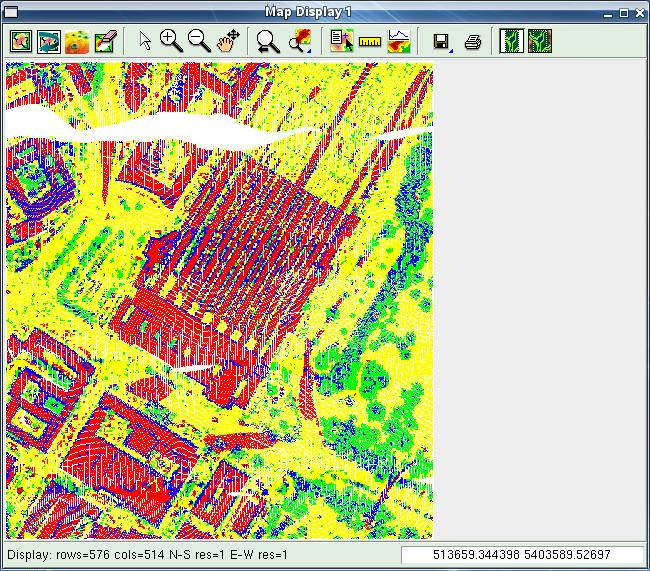
\includegraphics[width=0.75\textwidth]{images/correction}}}
    \end{picture}
  \end{minipage}
\end{frame}
%%==================================================================Sb
\subsection{\texttt{v.outlier}}
%%==================================================================F 
\begin{frame}[fragile,shrink=5]
  \frametitle{\path{v.outlier}}
  \begin{beamerboxesrounded}[shadow=true]{\textbf{\path{v.lidar.edgedetection}}
    \texttt{ input=name output=name outlier=name [soe=value] [son=value] 
    [lambda\_i=value] [thres\_o=value]}}
    \begin{itemize}
      \item \textbf{input}: name of the input vector map
      \item \textbf{output}: name of the output vector map
      \item \textbf{soe}: Interpolation spline step value in e-w direction
      \item \textbf{son}: Interpolation spline step value in n-s direction
      \item \textbf{lambda\_i}: Thychonov regularization weigth. (default: 0.1)
      \item \textbf{thres\_o}: Threshold for the outliers. (default: 50)
    \end{itemize}
  \end{beamerboxesrounded}
  %\pause
  \begin{beamerboxesrounded}[shadow=true]{Sintaxis}
\scriptsize
%\testcode
\begin{verbatim}
GRASS6 (stuttgart): > # Limpiamos el primer impulso
GRASS6 (stuttgart): > v.outlier in=stuttgart_first out=station_first \
> outlier=station_first_out soe=10 son=10 thres_o=25
GRASS6 (stuttgart): > # Limpiamos el ultimo impulso
GRASS6 (stuttgart): > v.outlier in=stuttgart_last out=station_last \
> outlier=station_last_out soe=10 son=10 thres_o=30
\end{verbatim}
\end{beamerboxesrounded}
\end{frame}
%%==================================================================Sb
\subsection{\texttt{v.lidar.edgedetection}}
%%==================================================================F 
\begin{frame}[fragile,shrink=10]
  \frametitle{\path{v.lidar.edgedetection}}
  \begin{beamerboxesrounded}[shadow=true]{\textbf{\path{v.lidar.edgedetection}}
    \texttt{ input=name output=name first=name see=value sen=value 
    [lambda\_g=value] [tgh=value] [tgl=value] [theta\_g=value] [lambda\_r=value]}}
   \begin{itemize}
    \item \textbf{input}: name of the input vector map
    \item \textbf{output}: name of the output vector map
    \item \textbf{see}: Interpolation spline step value in e-w direction
    \item \textbf{sen}: Interpolation spline step value in n-s direction
    \item \textbf{lambda\_g}: Regularization weight in gradient evaluation (default: 0.01)
    \item \textbf{tgh}: High gradient threshold for edge classification (default: 6)
    \item \textbf{tgl}: Low gradient threshold for edge classification (default: 3)
    \item \textbf{theta\_g}: Angle range for same direction detection (default: 0.26)
    \item \textbf{lambda\_r}: Regularization weight in residual evaluation (default: 2)
   \end{itemize}
  \end{beamerboxesrounded}
 %\pause
 \begin{beamerboxesrounded}[shadow=true]{Sintaxis}
\scriptsize
%\testcode
\begin{verbatim}
GRASS6 (stuttgart): > v.lidar.edgedetection in=station_last see=4 sen=4 \
> lambda_g=0.1 out=station_edge
\end{verbatim}
\end{beamerboxesrounded}
\end{frame}
%%==================================================================F 
%\pgfdeclareimage[width=0.65\textwidth]{edge}{images/edge}
%\begin{frame}
% \frametitle{Visualización de \LARGE\path{v.lidar.edgedetection}}
%\begin{columns}
%  \begin{column}{0.7\textwidth}
%    \begin{center}
%	\begin{tikzpicture}
%    	  \pgftext[bottom,left,at={\pgfpointxy{0}{0}}]{\pgfuseimage{edge}}
%	\end{tikzpicture}
%   \end{center}
%  \end{column}
%  \begin{column}{0.25\textwidth}
%	\begin{enumerate}
%	 \item \textcolor{red}{Borde}
%	 \item \textcolor{yellow!95!black}{Terreno}
%	\end{enumerate}
%  \end{column}
%\end{columns}
%\end{frame}
%%==================================================================Sb
\subsection{\texttt{v.lidar.growing}}
%%==================================================================F 
\begin{frame}[fragile,shrink=10]
  \frametitle{\path{v.lidar.growing}}
  \begin{beamerboxesrounded}[shadow=true]{\textbf{\path{v.lidar.growing}}
    \texttt{ input=name output=name first=name [tj=value] [td=value]}}
    \begin{itemize}
     \item \textbf{input}: name of the input vector map
     \item \textbf{output}: name of the output vector map
     \item \textbf{first}: name of the input vector map of the first pulse points
     \item \textbf{tj}: Threshold in planimetric units for considering two 
         measurements as corresponding first and double pulse. (default 0.2)
     \item td: Threshold in height units for classifying a point as double pulse. 
         (default: 0.6)
    \end{itemize}
  \end{beamerboxesrounded}
  %\pause
  \begin{beamerboxesrounded}[shadow=true]{Sintaxis}
\scriptsize
\begin{verbatim}
GRASS6 (stuttgart): > # Se disminuye primero la resolucion
GRASS6 (stuttgart): > g.region -p res=2
GRASS6 (stuttgart): > v.lidar.growing in=station_edge out=station_grow \
> first=station_first
\end{verbatim}
\end{beamerboxesrounded}
\begin{itemize}
 \item \alert{Importante!!} Bajar la resolución de la región
\end{itemize}
\end{frame}
%%==================================================================F 
%\pgfdeclareimage[width=0.65\textwidth]{grow}{images/grow}
%\begin{frame}
% \frametitle{Visualización de \LARGE\path{v.lidar.growing}}
%\begin{columns}
%  \begin{column}{0.65\textwidth}
%    \begin{center}
%	\begin{tikzpicture}
%    	  \pgftext[bottom,left,at={\pgfpointxy{0}{0}}]{\pgfuseimage{grow}}
%	\end{tikzpicture}
%   \end{center}
%  \end{column}
%  \begin{column}{0.35\textwidth}
%	\begin{enumerate}
%	 \item \textcolor{yellow!95!black}{Terreno}
%	 \item \textcolor{green}{Terreno doble eco}
%	 \item \textcolor{blue!90!black}{Objeto doble eco}
%	 \item \textcolor{red}{Objeto}
%	\end{enumerate}
%  \end{column}
%\end{columns}
%\end{frame}
%%==================================================================Sb
\subsection{\texttt{v.lidar.correction}}
%%==================================================================F 
\begin{frame}[fragile,shrink=5]
  \frametitle{\path{v.lidar.correction}}
  \begin{beamerboxesrounded}[shadow=true]{\textbf{\path{v.lidar.correction}}
    \texttt{ input=name  output=name  terrain=name  sce=value  scn=value 
    [lambda\_c=value]  [tch=value]  [tcl=value]}}
    \begin{itemize}
     \item \textbf{input}: name of the input vector map
     \item \textbf{output}: name of the output vector map
     \item \textbf{terrain}: name of the terrain output vector map
     \item \textbf{sce}: Interpolation spline step value in e-w direction
     \item \textbf{scn}: Interpolation spline step value in n-s direction
     \item \textbf{lambda\_c}: Regularization weight in reclassification evaluation. (default 1)
     \item \textbf{tch}: High difference threshold (terrain/object). (default 2)
     \item \textbf{tcl}: Low differnce threshold (object/terrain). (default 1)
    \end{itemize}
  \end{beamerboxesrounded}
  %\pause
  \begin{beamerboxesrounded}[shadow=true]{Sintaxis}
\scriptsize
\begin{verbatim}
GRASS6 (stuttgart): > v.lidar.correction in=station_grow sce=60 scn=60 \
> lambda_c=2 tcl=0.1 out=station_corr terrain=station_terr
\end{verbatim}
  \end{beamerboxesrounded}
\end{frame}
%%==================================================================F 
%\pgfdeclareimage[width=0.65\textwidth]{corr}{images/correction}
%\begin{frame}
% \frametitle{Visualización de \LARGE\path{v.lidar.correction}}
%\begin{columns}
%  \begin{column}{0.65\textwidth}
%    \begin{center}
%	\begin{tikzpicture}
%    	  \pgftext[bottom,left,at={\pgfpointxy{0}{0}}]{\pgfuseimage{corr}}
%	\end{tikzpicture}
%   \end{center}
%  \end{column}
%  \begin{column}{0.35\textwidth}
%	\begin{enumerate}
%	 \item \textcolor{yellow!95!black}{Terreno}
%	 \item \textcolor{green}{Terreno doble eco}
%	 \item \textcolor{blue!90!black}{Objeto doble eco}
%	 \item \textcolor{red}{Objeto}
%	\end{enumerate}
%  \end{column}
%\end{columns}
%\end{frame}
%%==================================================================S INTRODUCTION
\section{LAStools}
%%==================================================================F 
\begin{frame}
  \frametitle{LAStools}
  \begin{enumerate}
    \item LASlib es una librería para la \alert{lectura} y \alert{escritura} de archivos en el
      estándar ASPRS LAS en C++
    \item Comandos para gestionar, manipular, transformar y procesar datos LiDAR
      en formato LAS
    \item \alert{LAStools}
      \begin{itemize}
        \item lasground.exe, lasheight.exe, lasclassify.exe, lasoverlap.exe,
          lascontrol.exe, lasgrid.exe, lastile.exe, lassort.exe, Lasclip.exe,
          lasinfo.exe, lasindex.exe, lasthin.exe, las2las.exe, lasboundary.exe,
          lasduplicate.exe, las2tin.exe,las2dem.exe, las2iso.exe, lasmerge.exe,
          lassplit.exe, lasprecision.exe, las2shp.exe, shp2las.exe, lasview.exe,
          laszip.exe, las2txt.exe, txt2las.exe
        \item las2las.cpp, las2txt.cpp, lasdiff.cpp, lasindex.cpp, lasinfo.cpp,
          lasmerge.cpp, lasprecision.cpp, laszip,cpp, txt2las.cpp
      \end{itemize}
  \end{enumerate}
\end{frame}
%%==================================================================F 
\begin{frame}
  \frametitle{Licencia}
  \begin{enumerate}
    \item Parte libre y abierta
      \begin{itemize}
        \item LASlib (con LASzip)
        \item herramientas principales: las2las, las2txt, laszip,\ldots
        \item Licencia \alert{LGPL}
      \end{itemize}
    \item Parte privativa y cerrada
      \begin{itemize}
        \item No es libre excepto para fines académicos o educacionales (con
          límites)
        \item La versión completa se puede licenciar
      \end{itemize}
  \end{enumerate}
\end{frame}
%%==================================================================F 
\begin{frame}
  \frametitle{Historia}
  \begin{enumerate}
    \item Inicio del desarrollo en Enero de 2007
      \begin{itemize}
        \item API para lectura/escritura de LAS
        \item lasinfo, lasview, last2txt, txt2las, laszip, las2las
      \end{itemize}
    \item Publica desde Abril de 2007
    \item Aparece libLAS como un \emph{fork} en Diciembre de 2007
    \item Comercializada desde 2010
      \begin{itemize}
        \item GUI + multi-procesador en 2011
        \item ArcGIS toolbox desde Abril de 2012
      \end{itemize}
    \item En internet
      \begin{itemize}
        \item \beamergotobutton{\url{http://groups.google.com/group/lastools}}
        \item \beamergotobutton{\url{http://facebook.com/lastools}}
        \item \beamergotobutton{\url{http://twitter.com/lastools}}
        \item \beamergotobutton{\url{http://www.linkedin.com/groups?gid=4408378}}
      \end{itemize}
  \end{enumerate}
\end{frame}
%%==================================================================F 
  \defverbatim[colored]\laszip{
     \begin{lstlisting}[style=shell]
        $ laszip lidar.las lidar.laz
        $ laszip lidar.laz lidar_copy.las
    \end{lstlisting}
  }
\begin{frame}
  \frametitle{LASzip}
  \begin{enumerate}
    \item Compresión de archivos .LAS sin \alert{pérdida}
    \item 7\% - 20\% del tamaño del archivo original
    \item Ganador del premio Geospatial World Forum 2012 Technology 
      Innovation Award para el procesado de datos LiDAR
    \item Incorporado en: LAStools, Global Mapper, Opals (TU Wien)...
    \item Utilizado por: NOAA, USGS, Fugro, Blom, Riegl, Dielmo...
    \laszip
  \end{enumerate}
\end{frame}
%%==================================================================F 
  \defverbatim[colored]\gestion{
     \begin{lstlisting}[style=shell]
        $ for lasinfo lidar.las
        $ lasdiff lidar1.las lidar2.las
        $ lasmerge -i in1.las -i in2.las -i in3.las -o out.las
    \end{lstlisting}
  }
  \defverbatim[colored]\formato{
     \begin{lstlisting}[style=shell]
        $ las2txt -i lidar.las -o lidar.txt -parse xyzi
        $ txt2las -i lidar.taxyz -o lidar.las -parse xyzsi
        $ las2ogr -i mydata.las -o points.shp -f "ESRI Shapefile"
    \end{lstlisting}
  }
\begin{frame}
  \frametitle{LibLAS}
  Comandos (basados en LASTools) para gestionar, manipular, 
    transformar y procesar datos LiDAR en formato LAS
    \begin{itemize}
      \item Gestionar
        \gestion
      \item Cambio de formato
        \formato
    \end{itemize}
\end{frame}
%%==================================================================F 
  \defverbatim[colored]\liblas{
    \begin{lstlisting}[language=python,style=mio]
    >>> from liblas import file
    >>> f = file.File('file.las',mode='r')
    >>> for p in f:
    ...     print 'X,Y,Z: ', p.x, p.y, p.z
    \end{lstlisting}
  }
  \begin{frame}
  \frametitle{LibLAS}
  \begin{enumerate}
    \item Librería para la \alert{lectura} y \alert{escritura} de archivos en el estándar \alert{ASPRS LAS}
    \item Compilable
    \begin{itemize}
      \item C/C++
      \item Bindings: \alert{python}, C\#, VB.NET, Ironpython\ldots
        \liblas
    \end{itemize}
    \item Paquetes
    \begin{itemize}
      \item \alert{OSGeo4W}
      \item DebianGIS
    \end{itemize}
  \end{enumerate}
\end{frame}
%%==================================================================F 
\begin{frame}
  \frametitle{PDAL}
  \begin{enumerate}
    \item \alert{PDAL}: \alert{P}oint \alert{D}ata \alert{A}bstraction
            \alert{L}ibrary
    \item Biblioteca de funciones para la transformación de nubes de datos LiDAR
      a varios formatos (tipo GDAL)
    \item C++
    \item Licencia \alert{BSD}
    \item \beamergotobutton{\url{http://pointcloud.org/}}
    \item<2> \alert{¡NO CONFUNDIR CON PCL!}
  \end{enumerate}
\end{frame}
%%==================================================================F 
\begin{frame}
  \frametitle{PCL}
  \begin{enumerate}
    \item \alert{PCL}: \alert{P}oint \alert{C}loud \alert{L}ibrary
    \item Biblioteca de funciones para el procesado de nubes de datos en 3D
    \item Paquetes multiplataforma
    \item Licencia \alert{BSD}
    \item \beamergotobutton{\url{http://pointclouds.org/}}
    \item<2> \alert{¡NO CONFUNDIR CON PDAL!}
  \end{enumerate}
    \begin{picture}(350,90)
    \put(180,0){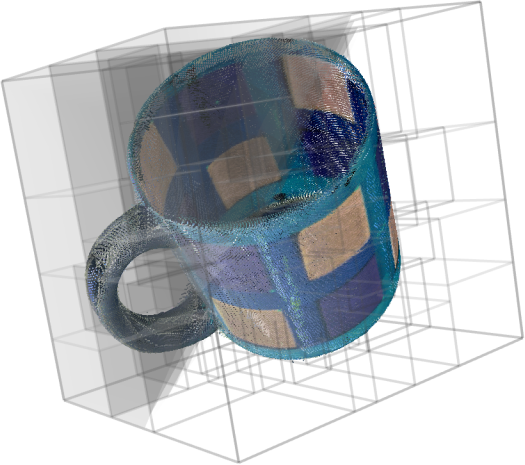
\includegraphics[width=0.45\textwidth]{images/mug}}
    \end{picture}
\end{frame}
%%==================================================================F 
\begin{frame}
  \frametitle{¡Datos LIBRES!}
  \begin{enumerate}
    \item \beamergotobutton{\url{http://www.lidar-online.com/products-list.php}}
    \item \beamergotobutton{\url{http://opentopo.sdsc.edu/gridsphere/gridsphere?cid=databases}}
    \item \beamergotobutton{\url{http://opentopography.org/}}
    \item \beamergotobutton{\url{http://liblas.org/samples/}}
    \item \beamergotobutton{\url{http://www.csc.noaa.gov/digitalcoast/data/chartstopobathy/download}}
    \item \beamergotobutton{\url{ftp://ftp.lmic.state.mn.us/pub/data/elevation/lidar/}}
  \end{enumerate}
      Muchos más en:
  \begin{enumerate}
    \item \beamergotobutton{\url{http://laszip.org/}}
  \end{enumerate}
\end{frame}
%%==================================================================F 
\begin{frame}
  \frametitle{Descarga de .LAZ}
  \begin{minipage}{0.35\textwidth}
  \begin{enumerate}[<+->]
    \item Open Topography
    \item Minnesota DNR
  \end{enumerate}
  \end{minipage}
    \begin{picture}(375,120)
    \uncover<1->{\put(170,-10){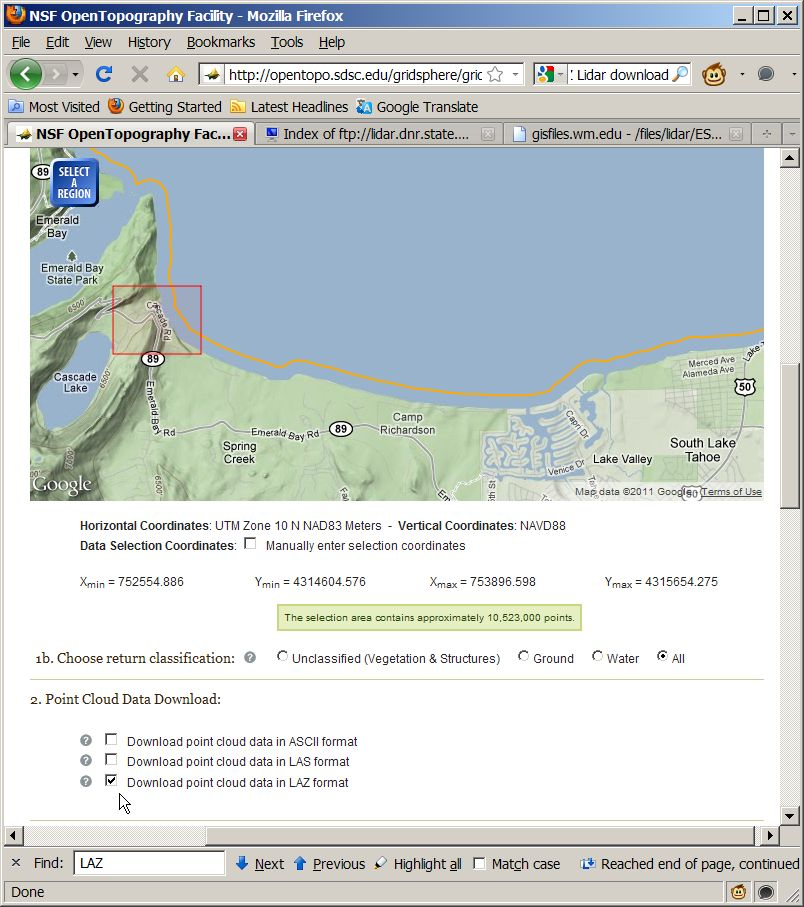
\includegraphics[width=0.48\textwidth]{images/open_topo}}}
    \uncover<2->{\put(170,-10){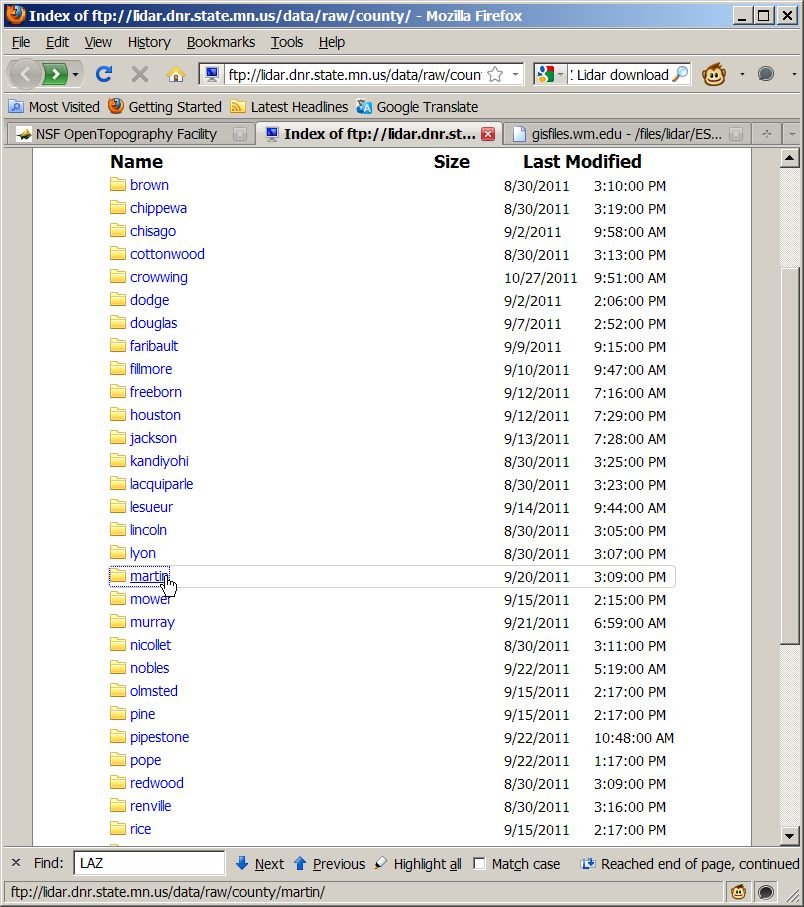
\includegraphics[width=0.48\textwidth]{images/minnesota}}}
    \uncover<3->{\put(170,-10){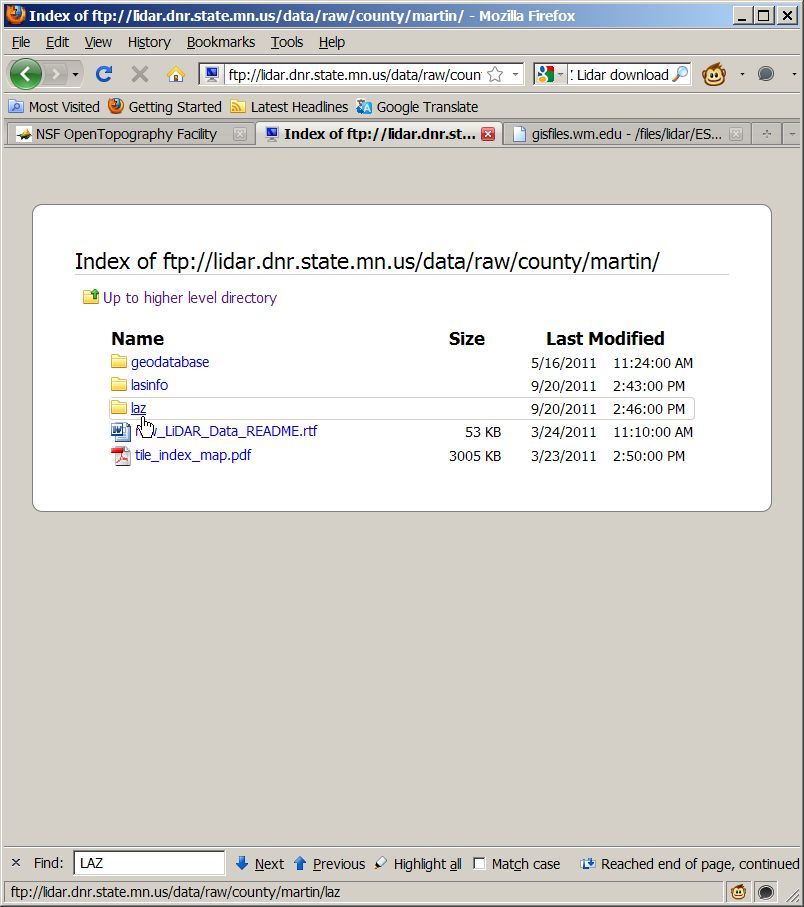
\includegraphics[width=0.48\textwidth]{images/minnesota_martin}}}
    \uncover<4->{\put(170,-10){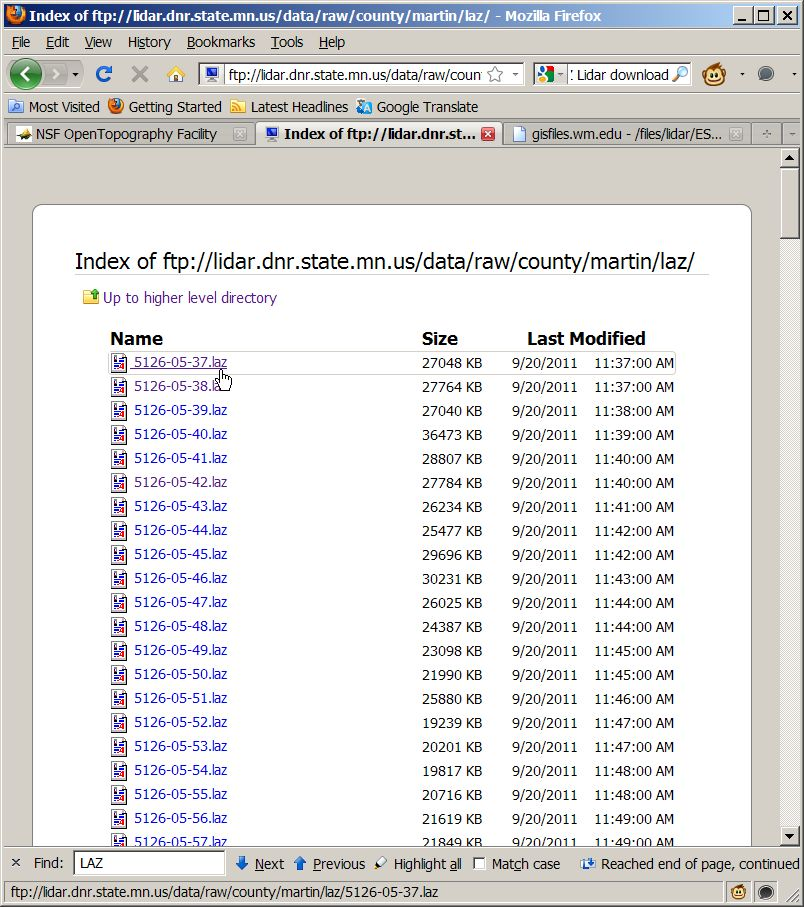
\includegraphics[width=0.48\textwidth]{images/minnesota_laz}}}
    \end{picture}
\end{frame}
%%==================================================================S 
\section{Procesamiento con LAStools}
%%==================================================================Sb
\subsection{Control de Calidad}
%%==================================================================F
  \defverbatim[colored]\calidad{
    \begin{lstlisting}[language=bash,style=shell]
C:\> # Resumen de todo el contenido de los archvios LAS
C:\> lasinfo -i *.las -compute_density
C:\> # Inspeccion visual de los LAS
C:\> lasview -i *.las 
C:\> # Calcular el contorno y los huecos del vuelo LiDAR
C:\> lasboundary  -i *.las  -holes  -disjoint  -oshp
C:\> # Crear una malla con la densidad puntual y visualizarla en falso color
C:\> lasgrid -i *.las  -density  -step 3  -set_minmax 0 20 -false  -opng  -utm 28N
C:\> # Determinar si existen puntos repetidos
C:\> lasduplicate  -i *.las  -unique_xyz  -onil
C:\> # Comprobar la alineacion vertical y horizontal de las pasadas
C:\> lasoverlap  -i *.las  -step 3
    \end{lstlisting}
  }
\begin{frame}
  \frametitle{Control de Calidad}
\calidad
\end{frame}
%%==================================================================F
  \defverbatim[colored]\preparacion{
    \begin{lstlisting}[language=bash,style=shell]
C:\> # Mejora de los datos y reproyeccion
C:\> las2las  -i *.las -rescale 0.01 0.01 0.01  -utm 28N  -olaz  -odix  l
C:\> # Unir todos los archivos y dividir los datos en teselas
C:\> lastile -i *l.laz  -tile_size 500  -buffer 30  -olaz  -o tiles
C:\> # Clasificar puntos terreno (class 2)
C:\> lasground  -i tiles*.laz  -fine  -olaz  -odix g
C:\> # Calcular la altura de los objetos respecto al terreno
C:\> lasheight  -i tiles*g.laz  -olaz  -odix h
C:\> # Clasificar los puntos no-terreno en edificios
C:\> # (class 6) y vegetacion (class 5)
C:\> lasclassify  -i tiles*gh.laz  -olaz  -odix c
C:\> # Calcular la altura de los objetos y 
C:\> # reemplazar la anterior
C:\> lasheight  -i tiles*ghc.laz  -replace_z  -olaz  -odix h
    \end{lstlisting}
  }
\begin{frame}
  \frametitle{Preparación de los datos}
\preparacion
\end{frame}
%%==================================================================F
  \defverbatim[colored]\derivados{
    \begin{lstlisting}[language=bash,style=shell]
C:\> # Triangular puntos en un TIN y un raster (DSM)
C:\> las2dem  -i tiles*.laz  -first_only  -step 2.5  -use_tile_bb  -otif
C:\> # Triangular puntos en un TIN y un raster (DTM)
C:\> las2dem  -i tiles*g.laz  -keep_class 2  -step 2.5  -use_tile_bb  -ocut 1  -otif
C:\> # Encontrar la altura maxima en cada celda y exportar a PNG
C:\> lasgrid  -i tiles*ghch.laz  -step 2.5  -use_tile_bb  -highest -false  -ocut 4  -opng
C:\> # Estimar la densidad de la vegetacion baja, media y alta
C:\> # contando los puntos por celda que caen en diferentes 
C:\> # intervalos de altura: 30cm-99cm; 1m-1.99m; 2m-3.99m
C:\> lasgrid  -i tiles*ghch.laz  -step 2.5  -clip_z 0.3 0.99  -density  -odix low  -oasc
C:\> lasgrid  -i tiles*ghch.laz  -step 2.5  -clip_z 1.0 1.99  -density  -odix mid1  -oasc
C:\> lasgrid  -i tiles*ghch.laz  -step 2.5  -clip_z 2.0 3.99  -density  -odix mid2  -oasc
    \end{lstlisting}
  }
\begin{frame}
  \frametitle{Cartografía derivada: Estudios Forestales}
\derivados
\end{frame}


%%==================================================================F
\againframe{portada}
%%==================================================================F

%\section{Resumen}
